\documentclass[a4paper]{article}
\usepackage[utf8]{inputenc}
\usepackage[german]{babel}
\usepackage[T1]{fontenc}
\usepackage[a4paper, margin=2cm, right=4cm]{geometry}
\usepackage{multirow}
\usepackage[hidelinks]{hyperref}
\usepackage{dirtytalk}
\usepackage{graphicx}
\usepackage{pdfcomment}
\usepackage{caption}
\usepackage[nomain, toc, section=section]{glossaries}
\usepackage[german, textwidth=3cm]{todonotes}
\usepackage{listings}
\usepackage{array}
\usepackage{ulem}
\usepackage{csquotes}
\usepackage[citestyle=verbose]{biblatex}
\usepackage[capposition=top]{floatrow}
\usepackage[titlesize=2em,parsize=1em,titlealign=r,nofullpage,clrpg]{colophon}

\graphicspath{ {./images/} }

\setlength{\marginparwidth}{3cm}

\title{Retron 5 - Retronlabo CFW User Guide, How-To und FAQ
\author{\url{https://github.com/jayp76}}
\thanks{Dank geht an ManCloud, Reminon und Stone}}

% so, we slightly abuse the glossary package here for the supported file types listing later. It kind of is that, in a way? It defines things that work with other things? Yay?
\newglossary[ftg]{file-type}{ftd}{ftn}{Dateiformate}

\newglossaryentry{ft:fba}{
  type=file-type,
  name=FBA,
  description={\texttt{*.zip}}
}
\newglossaryentry{ft:famicom}{
  type=file-type,
  name=Famicom,
  description={\texttt{*.fds}}
}
\newglossaryentry{ft:gb}{
  type=file-type,
  name=GameBoy,
  description={\texttt{*.gb} und \texttt{*.gbc}}
}
\newglossaryentry{ft:gg}{
  type=file-type,
  name=GameGear,
  description={\texttt{*.gg}}
}
\newglossaryentry{ft:gba}{
  type=file-type,
  name=GameBoy Advance,
  description={\texttt{*.gba}}
}
\newglossaryentry{ft:mdg}{
  type=file-type,
  name=MegaDrive/Genesis,
  description={\texttt{*.bin} und \texttt{*.md} und \texttt{*.gen}}
}
\newglossaryentry{ft:nes}{
  type=file-type,
  name=NES,
  description={\texttt{*.nes}}
}
\newglossaryentry{ft:ngp}{
  type=file-type,
  name=NeoGeoPocket,
  description={\texttt{*.ngp}}
}
\newglossaryentry{ft:pce}{
  type=file-type,
  name=PC-Engine,
  description={\texttt{*.pce}}
}
\newglossaryentry{ft:ps1}{
  type=file-type,
  name=PS1(PSX),
  description={zum Laden des Spieles \texttt{*.cue} ausw\"ahlen, ansonsten \texttt{bin+cue}}
}
\newglossaryentry{ft:mcd}{
  type=file-type,
  name=MegaCD/SegaCD,
  description={zum Laden des Spieles \texttt{*.cue} ausw\"ahlen, ansonsten \texttt{bin+cue}}
}
\newglossaryentry{ft:sms}{
  type=file-type,
  name=Master System,
  description={\texttt{*.sms}}
}
\newglossaryentry{ft:sfc}{
  type=file-type,
  name=Super Nintendo,
  description={\texttt{*.sfc} und \texttt{*.smc}}
}
\newglossaryentry{ft:ws}{
  type=file-type,
  name=Wonderswan,
  description={\texttt{*.ws} und \texttt{*.wsc}}
}

\makeglossaries

\setuptodonotes{}

\lstset{
  language=C++,
  numbers=left,
  numberstyle=\tiny,
  basicstyle=\footnotesize
}

\addbibresource{references.bib}

\begin{document}

\sffamily

\maketitle

\begin{abstract}
Dieser Guide beinhaltet nicht die Installationsschritte f\"ur die CFW, sondern nur das Handling mit Cartridges, Cores, Configs und Romsdumps.
\end{abstract}

\todo{Diesen Guide mit RetrolLabo Doku anreichern $\rightarrow$ ongoing}

\tableofcontents

\listoffigures

\listoftables

\colophontitle{Amige, Don't Read This Colophon!}
\begin{colophon}
... what are you doing. I told you explicitly NOT to! Now I need to actually come up with text for a colophon! Do you know how much copy you need to write for a colophon? Like, A FULL PAGE! ZOMG, THE HORROR!!\footnotemark

Uh... right... so... moving straight past that:

\emph{Why hello there!} I sure hope you are finding yourself to be having an excellent day, today. Certainly a good one for hacking your console to teach it new tricks! Don't worry, this is indeed the German version of this PDF. But I'm writing in English to highlight that I'm NOT the original author of this document - you should head on over to jayp76's github for that, yo!

BUT it is through the magicks of github and how that fosters collaboration, that I found this, liked it, wanted to help out by translating it, then noticed the PDF had no source - and no hyperlinks, meaning it was likely written in a word processor with a print to PDF function, and so there is no real source to collab on. And that's no good for a collaboration! Like, literally, by definition!

So... I translated it into LaTeX first, so I can procrastinate translating it into English - because Procrastination is For PROs, right? It's right in the word and all. But in all seriousness, translating a TeX file is much easier than a word document. For real.

I would like to point out that I have not actually proofread the text in here except for when I happened to notice a typo or somesuch - which, since it's German, ain't all that likely to be honest, cause I grew up in the South - we ain't speaking no German. It's literally a different language, and about as close to German as Dutch. So, if you find mistakes, however large: you get to keep both pieces. Pitch in and send a pull request with a fix. It's just LaTeX, it's not that hard.

You \emph{can DO IT}!

This was @EffinMaggie, and you go have a good day there now. Go apply what you read here into getting down with some new games on your Retron!

And stop reading colophons. They've not been hip since the 16th century. Like, you're gonna make FETCH happen before colophons are back in style, and after the time we've all had, YOU most DEFINITELY deserve yourself some FRESH STYLES! Have fun!

\end{colophon}

\footnotetext{... no, I don't have a thing going on about breaking style in otherwise meticulously crafted forms of publishing. That is a very specific thought, why would you think that? Have you been spying on my Twitter or Twitch? 'cause you shouldn't do that. At least not the Twitter - that's a terrible place. Made of terrible people. Like me. Also I broke a LaTeX package in the making of this joke, and you are probably never going to read this, unless you check the source. If you do: Good on you, mate! Well done! Curiosity might kill cats, but if you're reading English, you likely aren't one, so you're good, and learning! Huzzah!}

% neat hack to always page break between sections - thanks DuckDuckGo and David Carlisle for allowing me to find this. :)
\let\oldsection\section
\renewcommand\section{\clearpage\oldsection}
% additional note: we do this here instead of in the preamble, because we don't actually need to spread out all the different types of lists over a gazillion pages. We just want this for actual sections after the frontmatter.

\section{Welchen Mehrwert bringt die CFW?}

\begin{itemize}
  \item Neue und Alternative Cores z.B. PC-Engine
  \item Einfaches dumpen der eigenen Cartridges
  \item Laden eigener Rom dumps
  \item ggf. neue oder aktuellere Cores in Zukunft nachr\"ustbar
\end{itemize}

\todo{RetronLabo Doku auf SD Karte anpassen und ggf. als zip anh\"angen.}

\section{Welche Dateien werden f\"ur die aktuelle Retronlabo Firmware f\"ur die neuen und alternativen Cores ben\"otigt?}

\begin{figure}[h]
\caption{Screenshot einer Ordneransicht mit BIOS-Dateien}
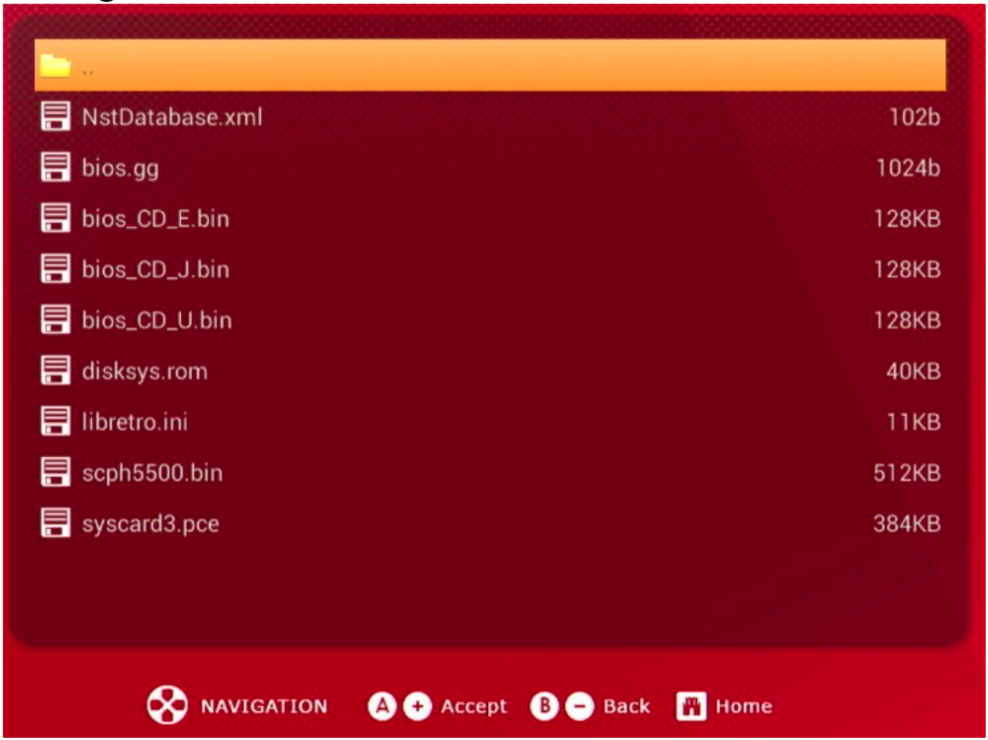
\includegraphics[width=\textwidth]{needed-files-for-alternate-cores}
\label{fig:needed-files-for-alternate-cores}
\floatfoot{Der Screenshot zeigt folgende Dateien: \texttt{NstDatabase.xml}, \texttt{bios.gg}, \texttt{bios\_CD\_E.bin}, \texttt{bios\_CD\_J.bin}, \texttt{bios\_CD\_U.bin}, \texttt{disksys.rom}, \texttt{libretro.ini}, \texttt{scph5500.bin}, \texttt{syscard3.pce.}}
\end{figure}

\begin{itemize}
  \item Die Dateien liegen auf der SD-Karte im \say{\#Config} Ordner und werden alle einzeln aber einmalig \"uber das Menu kopiert und bleiben nach einem Reboot erhalten. Diese landen im Ordner \say{\#Internal storage/\#Config}
\end{itemize}

\subsection{Anmerkungen}

\begin{itemize}
  \item NstDatabse.xml wird vom Nestopia f\"ur Famicom Disk System ben\"otigt
  \item libretro.ini wird f\"ur alle neuen und alternativen Cores ben\"otigt.
  \item Achtung: Geladene Cores werden hier und auch sonst im Menu \emph{nicht} angezeigt.
  \item neogeo.zip bleibt im FBA Spiele Verzeichnis und wird \emph{nicht} aus \say{\#Cores} kopiert
\end{itemize}

\section{Bios MD5sums}

Andere Bios k\"onnten auch funktionieren, aber hier, in Tabelle \ref{tbl:bios-files}, findet ihr die MD5sums der Bios Dateien mit denen ich Erfolg hatte.

\begin{table}
\begin{tabular}[t]{|l|>{\ttfamily}l|>{\ttfamily}r|}
  \hline
  \multicolumn{1}{|l}{\bfseries System} & \multicolumn{1}{c}{\bfseries Datei} & \multicolumn{1}{c|}{\bfseries Pr\"ufsumme} \\
  \hline
  Game Gear & bios.gg & 672E104C3BE3A238301ACEFFC3B23FD6 \\
  \multirow{3}{*}[1em]{MegaDrive/MegaCD} & \sout{bios\_CD\_E.bin} & \sout{7E146768A62DA68D771ED8B08079A5B5} \\
  & bios\_CD\_J.bin & 45DD7A6A87CA6AD4D0A54E8A2E3C097E \\
  & \sout{bios\_CD\_U.bin} & \sout{3B7D1CCA456F3CD7DFDF5C2711443D67} \\
  NES & disksys.rom & C8B78295EB182F25C90DCD3DB9FA81EC \\
  PS1 & scph5500.bin & 924E392ED05558FFDB115408C263DCCF \\
  PC-Engine & syscard3.pce & C00A65C9CC8707F7202CD15A091C6A3F \\
  \hline
\end{tabular}
\captionof{table}{Funktionierende BIOS-Dateien mit MD5 Pr\"ufsummen}
\label{tbl:bios-files}
\end{table}

\subsection{Anmerkungen}

\begin{itemize}
  \item PS1 Bios ist eigentlich das US Bios scph5501.bin, nur umbenannt damit der Core mit US Spielen funktioniert, ansonsten w\"aren mit scph5500.bin nur japanische Spiele m\"oglich.
  \item Das US Mega CD Bios wird trotz der Doku von RetronLabo nicht geladen. Aber das oben genannte Mega CD Bios mit oben genannter MD5sum ist Region Free. Oder man benennt das US Bios in das japanische um. Ggf. muss man die Konsole neu starten und das File neu kopieren und die Savegames/Snapshots auf der SD Karte l\"oschen.
  \item F\"ur den GameGear Core wird Laut RetronLabo Doku ein Bios ben\"otigt. Ihr m\"usst nach Majesco Game Gear suchen, da nicht alle GameGear mit einem Bios ausgestattet wurden. Weitere Infos dazu unter \footcite{ref:smsp-bios}.
\end{itemize}

\section{Alternativen Core laden}

\say{Load Rom} $\rightarrow$ \say{\#Cores} $\rightarrow$ System z.B. FBA $\rightarrow$ libcore-xxx.so z.B. libcore-fba.so $\rightarrow$ \say{Copy}

\subsection{Anmerkungen}

Alternative Cores werden nicht dauerthaft gespeichert und nach einen Reboot des Retron5 sind wieder die Standard Cores aktiv.

\emph{Muss man jedesmal rebooten um einen neuen Core zu laden?} Eigentlich nicht, ausser das System verh\"alt sich komisch oder nicht wie erwartet.

Falls es mal Probleme gibt ein Spiel zu laden, dann kann man unter \say{\texttt{\#Internal storage}/\texttt{der geladene Core}/\texttt{Spielename}} \"uber das Men\"u das geladen Spiel l\"oschen und danach ein neues Spiel laden. Siehe Screenshot \ref{fig:unknown-game}.

\begin{figure}[h]
\caption{Screenshot der Menu-Optionen zu einem ROM.}
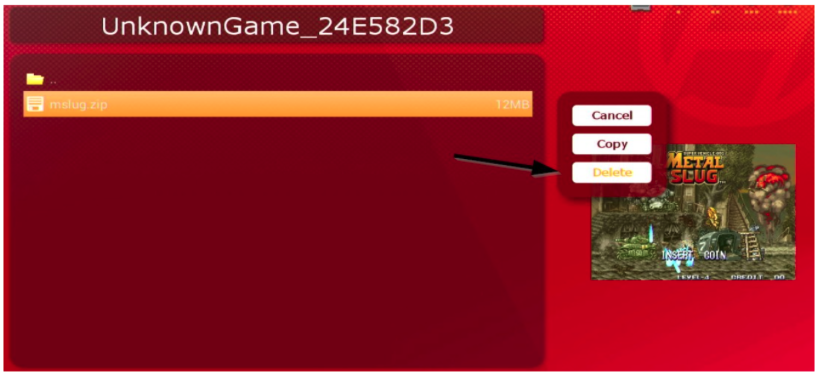
\includegraphics[width=\textwidth]{unknown-game}
\label{fig:unknown-game}
\floatfoot{Screenshot von einem pausierten Metal Slug das vom System nicht erkannt wurde. Ein Pfeil zeigt auf die \say{Delete} Menu-Option zu dem ROM.}
\end{figure}

\todo{Unbekannte Spielenamen einpflegen}

\section{Troubleshooting}

\begin{itemize}
  \item Wenn man einen Core l\"adt und startet danach das Spiel, aber man wird st\"andig ins Menu zur\"uckgeworfen, dann fehlt vermutlich das passende Bios und config Datei. Pr\"uft Anhand des Screenshots oben welche Dateien fehlen. Pr\"uft ggf. Datei Namen und MD5 Checksummen.
  \item Das Spiel l\"adt, aber macht was komisches. \\
Da der Retron5 immer ein Savestate des aktuell geladenen Spieles anlegt, kann das mit einem alternativen Core kollidieren. Z.B. wenn man das Spiel bisher mit dem Standard FDS Core gespielt hat, aber aus versehen Nestopia Core l\"adt. Dann reicht es in der Regel das Spiel \"uber das In-Game Menu zu resetten. Man muss nicht den Retron 5 rebooten.
  \item FBA Spiele zeigen nur ein schwarzes Bild aber der Ton ist zu h\"oren. \\
Ihr m\"usst folgendes in den Settings einstellen: \\
\say{Settings} $\rightarrow$ \say{Video} $\rightarrow$ \say{Force Original Resolution} $\rightarrow$ \say{On}
  \item Manchaml gibt es beim Playstation Core nach einer gewissen Spielzeit keinen Ton mehr. Manchmal hilft es das Spiel zu verlassen und neu zu starten und der Savestate neu geladen wird. Oder manuell einen selbst erstellten Savestate laden.
  \item L\"auft das Spiel zu schnell? Pr\"uft im den \say{Settings} ob die \say{Screen Refresh Rate} f\"ur PAL oder NTSC Spiel passt. Falls die Einstellung \say{Match Game} Probleme macht, dann stellt entsprechend auf \say{Force 60Hz} oder \say{Force 50Hz} ein. Beispiel: PSX Spiel \say{Ghost in the Shell PAL} l\"auft zu schnell wenn \say{Match Game} Refresh rate eingestellt ist und crashed manchmal die ganze Konsole. Mit \say{Force 50Hz} passt die Geschwindigkeit und es l\"auft stabiler.
  \item Das Spiel startet wegen einem fehlerhaften Savestate nicht der automatisch angelegt worden ist. Man kann diese Savestate \say{Snapshots} l\"oschen. Zu finden unter \say{SD Karte/Retron/Saves/Snapshot/System}. Manuell erstellte Savestates landen unter \say{SD Karte/Retron/Saves/Snapshot/User}
\end{itemize}

\glsaddallunused
\printglossary[title=Dateiformate, toctitle=Unterst\"utzte Dateiformate f\"ur ROMs, type=file-type, nonumberlist]

\section{Besonderheiten zum MegaCD/SegaCD Core}

In der \texttt{*.cue} Datei muss der Pfad zur Binary Datei angepasst werden. (F\"ur den PS1 Core scheint das nicht notwendig zu sein.) \\
Hier ein Beispiel: \\
\begin{lstlisting}[breaklines]
FILE "../../../../external_sd/Retron/Roms/Genesis/Batman Returns (Sega CD) (U).bin" BINARY
\end{lstlisting}

Hat man ein Image mit weiteren separaten Daten/Musik Dateien, dann muss f\"ur jeden Track der gleiche Pfad noch hinzugef\"ugt werden. \\
Beispiel: \\
\begin{lstlisting}[breaklines=true]
FILE "../../../../external_sd/Retron/Roms/Genesis/Popful Mail/Popful Mail (USA) (Track 1).bin "BINARY TRACK 01 MODE1 / 2352
INDEX 01 00:00:00
FILE "../../../../external_sd/Retron/Roms/Genesis/Popful Mail/Popful Mail (USA) (Track 2).bin" BINARY TRACK 02 AUDIO
INDEX 00 00:00:00
INDEX 01 00:02:00
FILE "../../../../external_sd/Retron/Roms/Genesis/Popful Mail/Popful Mail (USA) (Track 3).bin" BINARY TRACK 03 AUDIO
INDEX 00 00:00:00
INDEX 01 00:02:00
FILE "../../../../external_sd/Retron/Roms/Genesis/Popful Mail/Popful Mail (USA) (Track 4).bin" BINARY TRACK 04 AUDIO
INDEX 00 00:00:00
INDEX 01 00:02:00
\end{lstlisting}

\subsection{Anmerkung}

F\"ur SegaCD/MegaCD Spiele k\"onnen im \say{Retron5/Roms/Genesis} Ordner auf der SD Karte Unterordner erstellt werden. Leider funktioniert das \emph{nicht} f\"ur den Playstation 1 Core.

% \section{ROM Dumping}
\todo{Dumping FAQ/Anleitung}

\listoftodos[To-Do]

\printbibliography

\end{document}
